\section{Parte frontal} 

A parte frontal da estrutura comporta a roda dianteira da bicicleta e é responsável pela elevação e descida da plataforma dando a sensação de um terreno com variação de altura para que o usuário tenha uma experiência mais imersiva ao ambiente virtual.

    \begin{center}
    	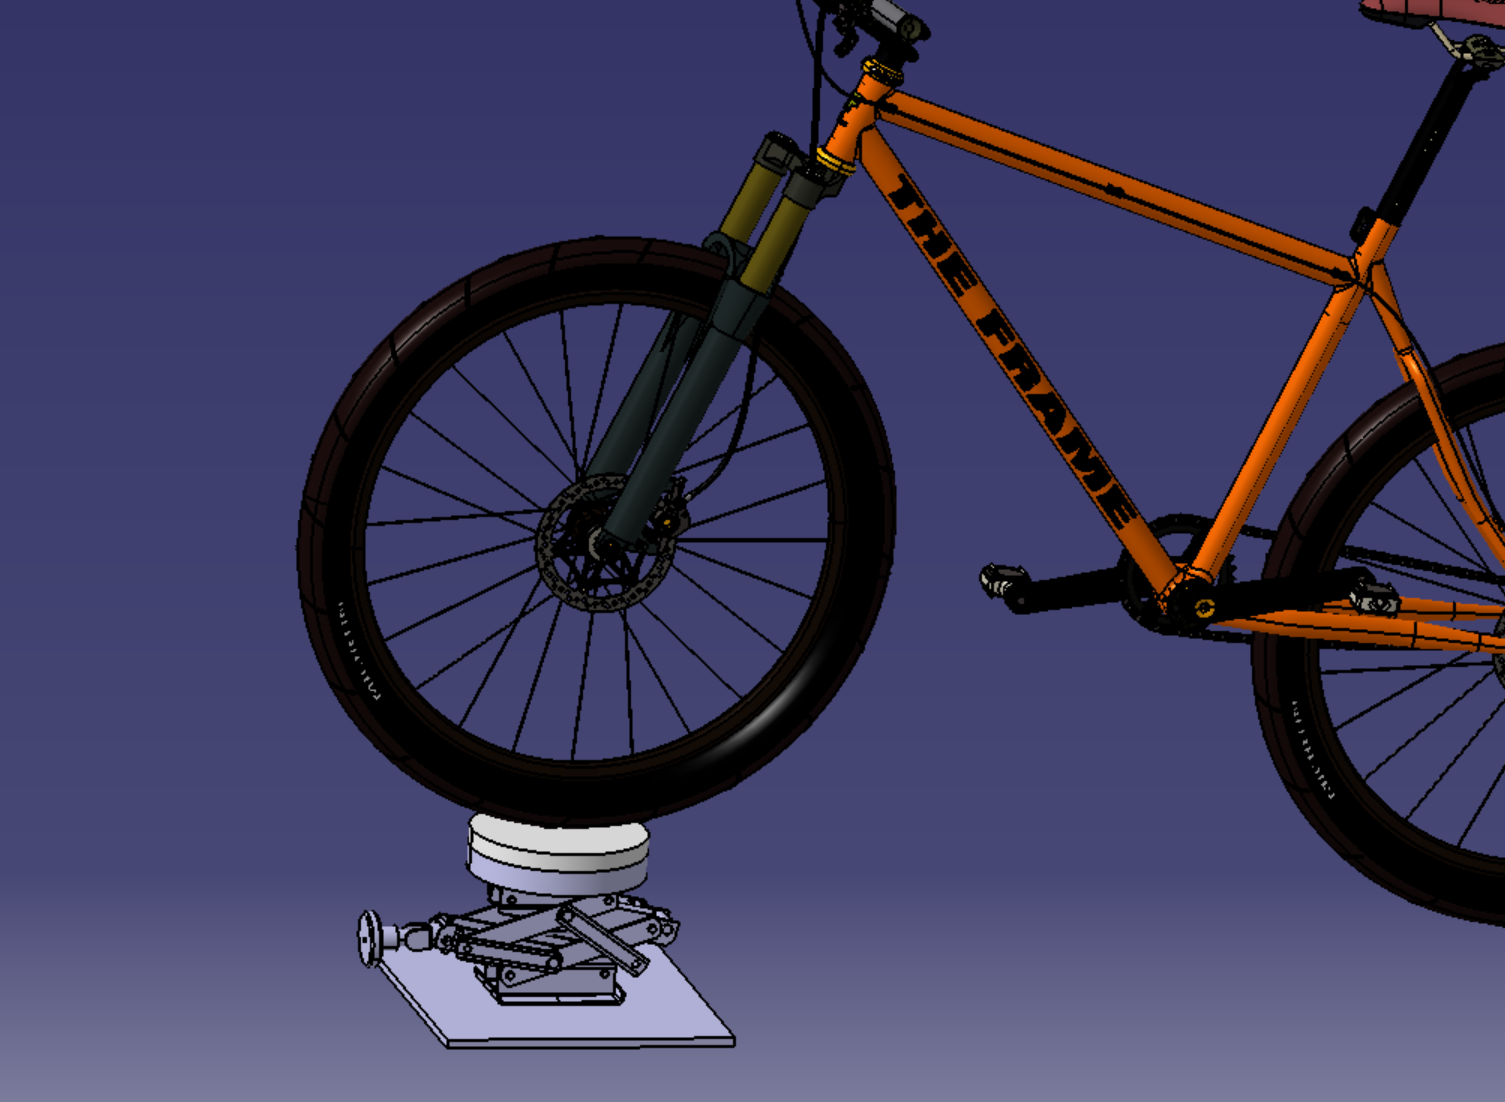
\includegraphics[scale=0.4]{figuras/partedafrente.png}
        \captionof{figure}{CAD da estrutura dianteira}
        \label{partedafrente}
    \end{center}

    Como anteriormente definido a esta parte fronta comporta:
    \begin{itemize}
        \item Macaco de elevação - acionado eletricamente por um motor com redução para suportar o peso do usuário e da estrutura complementar.

        \item Mesa giratória – Usinada para ser acoplada ao macaco e suportar os esforços de peso, composta por 3 peças
            \begin{itemize}
                \item Base inferior – Acoplada a base do macaco e onde ocorre o acoplamento ‘fêmea’ do rolamento e furo para abrigar potenciômetro;
                \item Rolamento;
                \item Base superior – Acoplada como "macho" no rolamento e sustentando a roda dando segurança e permitindo o giro do guidão controlando jogo
            \end{itemize}
    \end{itemize}    


\subsection{Mesa Giratória}

    \begin{center}
    	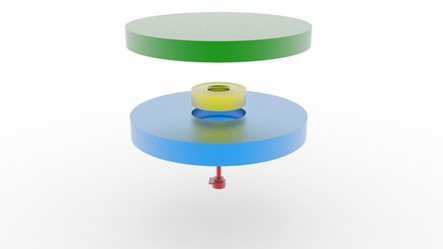
\includegraphics[scale=0.7]{figuras/acoplamento_frontal}
        \captionof{figure}{Esquema de acoplamento da parte frontal}
        \label{acoplamento_frontal}
    \end{center}
    
    \begin{center}
    	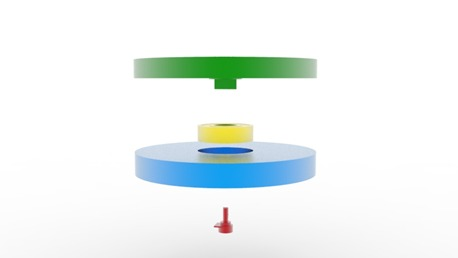
\includegraphics[scale=0.7]{figuras/acoplamento_frontal_2}
        \captionof{figure}{Outra vista do esquema de acoplamento}
        \label{acoplamento_frontal_2}
    \end{center}


    Tendo em vista o planejamento final de "assembly" da montagem final, começou-se o dimensionamento das peças a serem fabricadas.

    Para calcular os esforços para as simulações foram feitos os cálculos abaixo

    \begin{center}
    	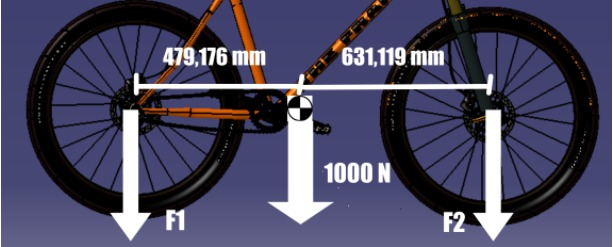
\includegraphics[scale=0.7]{figuras/analise_corpos_livres}
        \captionof{figure}{Análise de Corpos Livres}
        \label{analise_corpos_livres}
    \end{center}


    Como não há um padrão para distância entre os eixos e no centro de massa, medimos as distâncias da bicicleta que usamos nos desenhos em CAD. Com elas, utilizou-se conhecimentos básicos em estática para calcular a força resultante em cada roda. 

    Utilizando como momento nulo o centro da roda traseira e considerando que toda a plataforma mais o usuário gerem uma força de 1000 N, temos que:

\begin{equation}\label{eq290}
	\sum F = 0 
\end{equation}

 \begin{equation}\label{eq291}
	F2 \cdot 1110,295 - 1000 \cdot 479,176 = 0 
\end{equation}

 \begin{equation}\label{eq292}
	F2 = ~431,6 N
\end{equation}

 \begin{equation}\label{eq293}
	F1 =~ 568,4 N
\end{equation}

    Como a bicicleta varia sua inclinação em um ângulo muito pequeno, podemos aproximar para essa força em todo o percurso.

    Com as forças definidas foram feitas as simulações nas duas peças a serem usinadas no software ANSYS para avaliação dos resultados, validação e posterior usinagem.

    Para a parte superior da mesa foram feitas tais simulações:

     \begin{center}
    	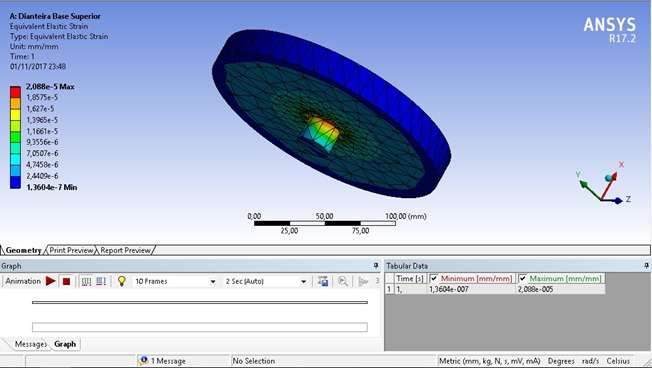
\includegraphics[scale=0.7]{figuras/sim_estatica_1}
        \captionof{figure}{Simulação estática estrutural – Tensão elástica equivalente}
        \label{sim_estatica_1}
    \end{center}

    %Figura 3: Simulação estática estrutural – Tensão elástica equivalente
    
     \begin{center}
    	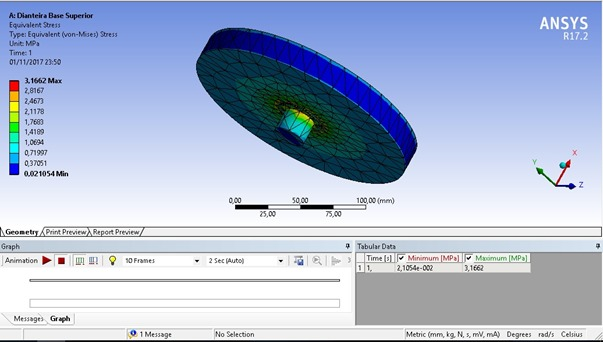
\includegraphics[scale=0.7]{figuras/stress_1}
        \captionof{figure}{Stress equivalente com Tensão de escoamento da mesa superior}
        \label{stress_1}
    \end{center}
   
    %Figura 4: Stress equivalente com Tensão de escoamento

     \begin{center}
    	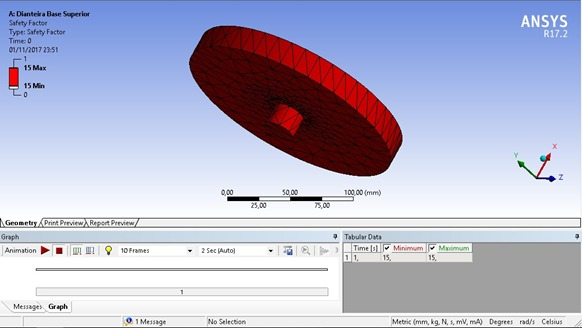
\includegraphics[scale=0.7]{figuras/fator_seguranca_1}
        \captionof{figure}{Fator de segurança da mesa superior}
        \label{fator_seguranca_1}
    \end{center}
    
    %Figura 5: Fator de segurança

     \begin{center}
    	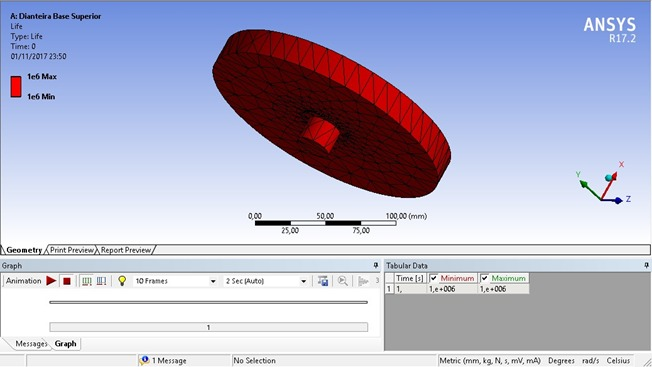
\includegraphics[scale=0.7]{figuras/vida_util_1}
        \captionof{figure}{Vida útil da mesa superior}
        \label{vida_util_1}
    \end{center}

    %Figura 6: Vida útil

    Como pode ser observado, todos os testes validam a peça para fabricação:

    \begin{itemize}
        \item A (figura \ref{sim_estatica_1}) mostra a deformação máxima (em mm) que a peça sofre com a carga aplicada e esta deformação é quase nula;
        \item A (figura \ref{stress_1}) mostra a tensão de escoamento que o material alcança (3,1662 MPa), sendo muito inferior a tensão de escoamento do aço 1045 (310 Mpa);
        \item A (figura \ref{fator_seguranca_1}) mostra o Fator de segurança da peça pelas condições de contorno, sendo esse fator igual a 15;
        \item A (figura \ref{vida_util_1}) mostra a vida útil da peça tendo como resultado uma peça com vida útil muito grande.
    \end{itemize}
  
    Conclui-se que essas peças são validadas para usinagem pois suportam com segurança os esforços nela aplicado. É possível observar que é uma peça superdimensionada, mas como um dos objetivos do projeto é a segurança do usuário e o macaco suporta o peso este fato é descartado.

    Para a parte inferior da mesa foram feitas tais simulações:

    \begin{center}
    	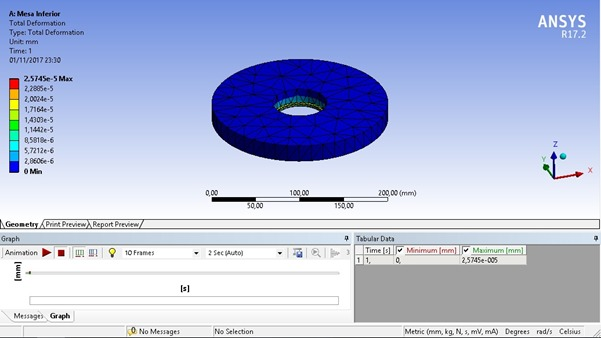
\includegraphics[scale=0.7]{figuras/modal_corpo_livre_1}
        \captionof{figure}{Modal de corpo livre - Deformação total }
        \label{modal_corpo_livre_1}
    \end{center}
    %Figura 7: Modal de corpo livre - Deformação total 

    \begin{center}
    	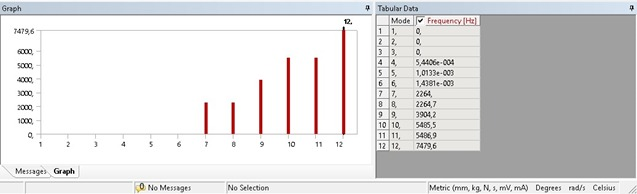
\includegraphics[scale=0.7]{figuras/ressonancia_1}
        \captionof{figure}{Módulos de vibração de ressonância da peça}
        \label{ressonancia_1}
    \end{center}
    %Figura 8: Módulos de vibração de ressonância da peça
    
    \begin{center}
    	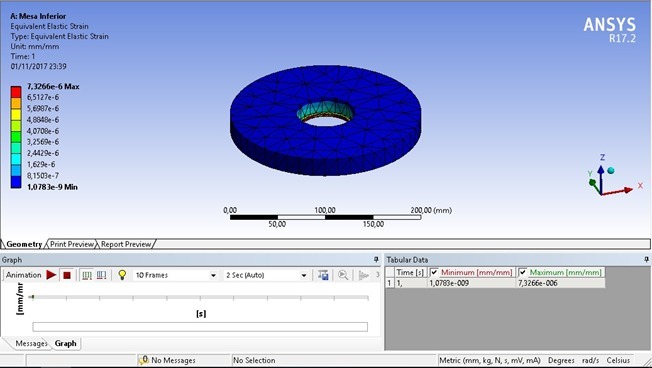
\includegraphics[scale=0.7]{figuras/sim_estatica_2}
        \captionof{figure}{Simulação estática estrutural – Tensão elástica equivalente}
        \label{sim_estatica_2}
    \end{center}
    %Figura 9: Simulação estática estrutural – Tensão elástica equivalente
    
    \begin{center}
    	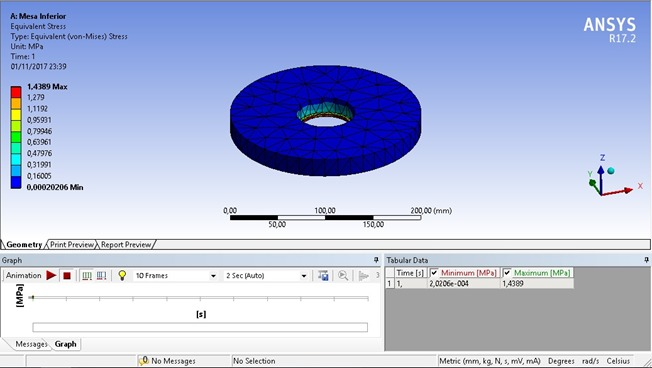
\includegraphics[scale=0.7]{figuras/stress_2}
        \captionof{figure}{Stress equivalente com Tensão de escoamento}
        \label{stress_2}
    \end{center}
    %Figura 10: Stress equivalente com Tensão de escoamento
    
    \begin{center}
    	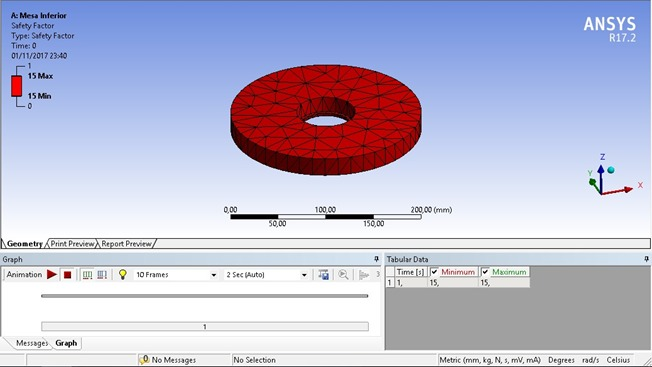
\includegraphics[scale=0.7]{figuras/fator_seguranca_2}
        \captionof{figure}{Fator de Segurança}
        \label{fator_seguranca_2}
    \end{center}
    %Figura 11: Fator de segurança
    
    \begin{center}
    	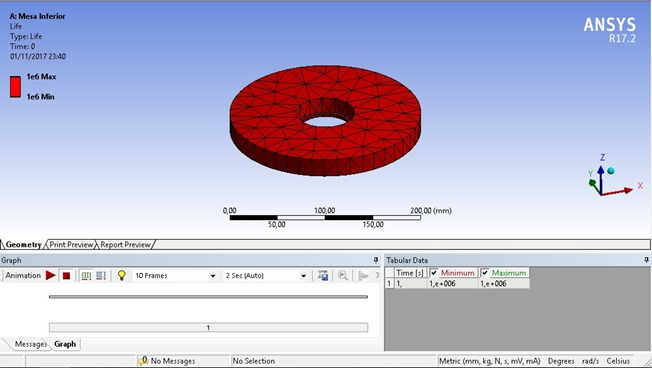
\includegraphics[scale=0.7]{figuras/vida_util_2}
        \captionof{figure}{Vida útil}
        \label{vida_util_2}
    \end{center}
    %Figura 12: Vida útil

    Como pode ser observado, todos os testes também validam a peça para fabricação:
    \begin{itemize}
        \item A (figura \ref{modal_corpo_livre_1} e  \ref{ressonancia_1}) mostram os resultados da análise modal de corpo livre mostrando a deformação total que as frequências causariam, que novamente são quase nulas, e as valores os quais a peça entra em ressonância, não tendo impacto pois a frequência gerada pelo macaco não conflita com nenhum dos valores atingidos
        \item A (figura \ref{sim_estatica_2}) mostra a deformação máxima (em mm) que a peça sofre com a carga aplicada e esta deformação é quase nula;
        \item A (figura \ref{stress_2}) mostra a tensão de escoamento que o material alcança (1,4389 MPa), sendo também muito inferior a tensão de escoamento do aço 1045 (310 Mpa);
        \item A (figura \ref{fator_seguranca_2}) mostra o Fator de segurança da peça pelas condições de contorno, sendo esse fator também igual a 15;
        \item A figura (figura \ref{vida_util_2}) mostra a vida útil da peça tendo como resultado uma peça com vida útil muito grande.
    \end{itemize}

    \begin{center}
    	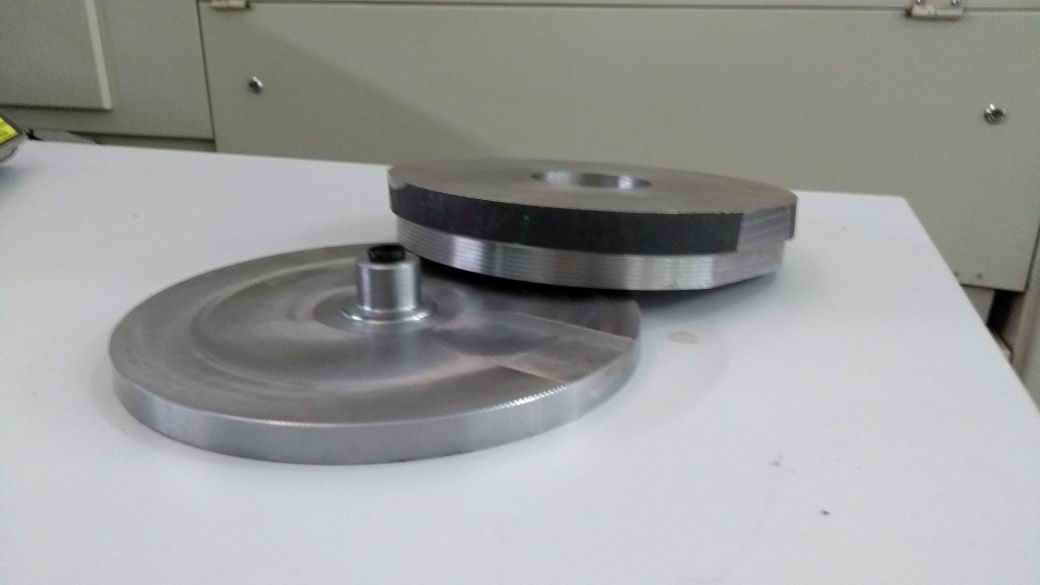
\includegraphics[scale=0.4]{figuras/mesa_giratoria_1}
        \captionof{figure}{Mesa giratória usinada}
        \label{mesa_giratoria_1}
    \end{center}
    %Figura 12: Mesa giratória usinada

    Esta peça também foi validada para usinagem pois suportam todos os esforços exigidos e nenhum fator oferece risco algum ao usuário. Esta peça também é superdimensionada mas, como explicado na outra peça, isso não oferece nenhuma perda ao projeto e o resultado final

\subsection{Macaco de Elevação}

  Com a exigência de fazer a elevação durante a simulação, foi projetado a utilização de um macaco que esticaria ao total 230 mm. Isso dá em torno de 6 graus de subida e 6 de descida. O motor que necessário para gerar a subida e descida da plataforma  tem elevada dimensões e peso bem maior que a do macaco tornando a fixação do motor ao macaco complexa, por sugestão do professor Rhander, escolheu-se comprar um macaco elétrico, da figura \ref{macaco_eletrico_1}, pois é uma solução viável dentro do orçamento disponível.

    \begin{center}
    	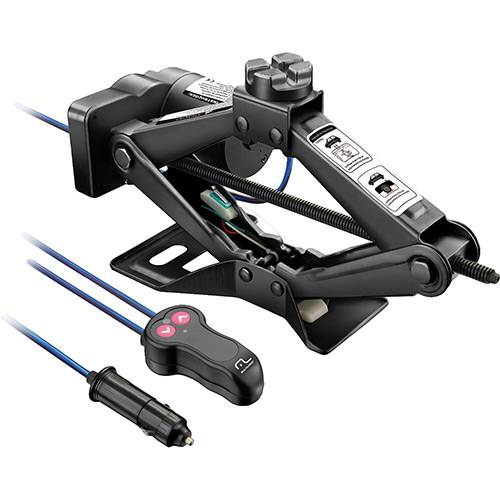
\includegraphics[scale=0.5]{figuras/macaco_eletrico_1}
        \captionof{figure}{Macaco com motor elétrico}
        \label{macaco_eletrico_1}
    \end{center}    
    %Figura 12: Macaco com motor elétrico

\section{Parte Traseira}
    A parte traseira da plataforma garante a interação com a realidade aumentada através de sensores de velocidade, controle de peso na pedalada para simular subida e geração de energia com um alternador. É adaptável a diferentes tamanhos de bicicleta.
 
    \begin{center}
    	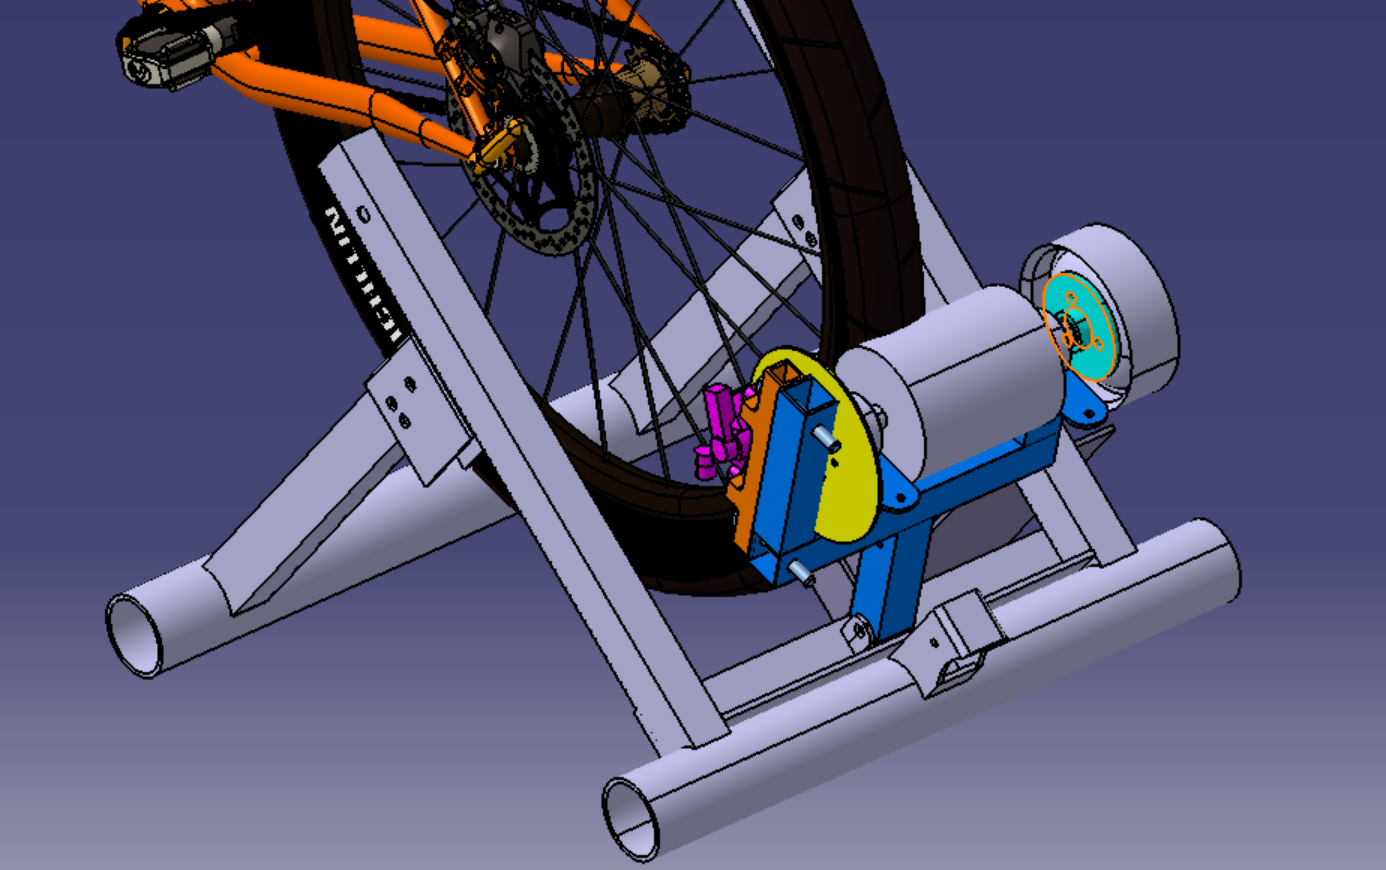
\includegraphics[scale=0.5]{figuras/parte_traseira}
        \captionof{figure}{CAD da parte traseira}
        \label{parte_traseira_1}
    \end{center}    
    %Figura X: CAD da parte traseira

    O esqueleto, estrutura em cinza, foi adquirido de um projeto antigo no galpão que usava para fins semelhantes. Adaptado a ele, foram projetados o suporte do freio e do alternador. Após estar operacional, serão reajustados algumas peças de tal esqueleto que estão velhas ou em condições não ideais.

\subsection{Cavalete de sustentação}

    A estrutura traseira comporta a roda traseira da bicicleta, acoplando-as por fusos com um acoplador nas pontas que encaixa na bicicleta exatamente no eixo da roda. Essa estrutura tem como objetivo sustentar a bicicleta e comportar o rolete traseiro onde haverá o sistema de freio e gerador de energia.

    Como anteriormente definido a esta parte traseira comporta:
    \begin{itemize}
        \item Duas peças que juntas se tornam um cavalete.
    \end{itemize}
    
    \begin{center}
    	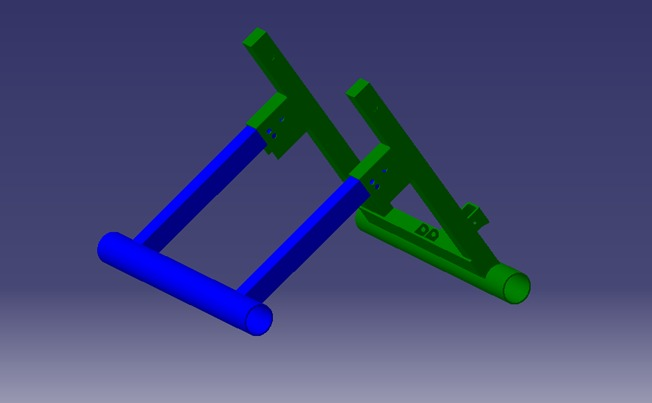
\includegraphics[scale=0.7]{figuras/esquema_traseira_1}
        \captionof{figure}{Esquema estrutura parte traseira}
        \label{esquema_traseira_1}
    \end{center}    
    %Figura 1: Esquema estrutura parte traseira

    \begin{center}
    	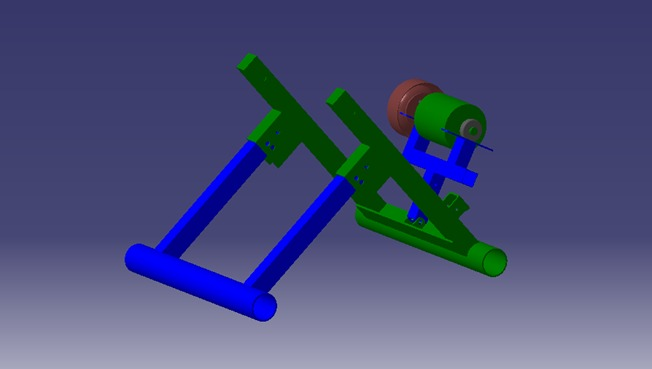
\includegraphics[scale=0.7]{figuras/parte_traseira_2}
        \captionof{figure}{Esquema estrutura completa de acoplamento parte traseira.}
        \label{parte_traseira_2}
    \end{center}        
    %Figura 2: Esquema estrutura completa de acoplamento parte traseira.
   
    \begin{center}
    	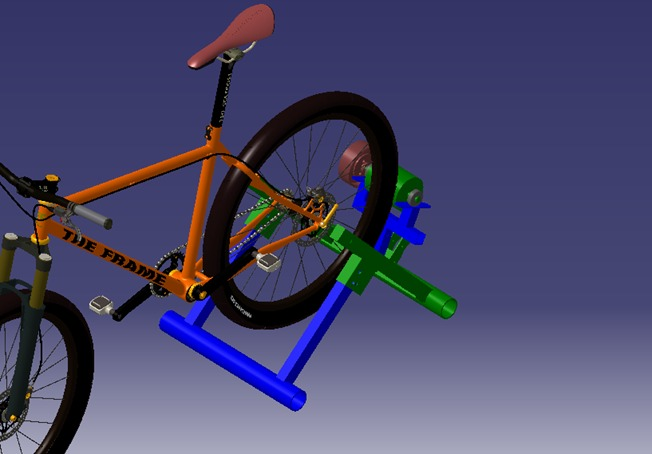
\includegraphics[scale=0.7]{figuras/acoplamento_est_1}
        \captionof{figure}{Acoplamento estrutura em uma bicicleta.}
        \label{acoplamento_est_1}
    \end{center}      
    %Figura 3: Acoplamento estrutura em uma bicicleta.
  
    Para calcular os esforços para as simulações, foram usados os cálculos apresentados na figura \ref{analise_corpos_livres} - Análise de Corpos Livres”.  Nesse caso as análises foram feitas com uma força de 2200 N para aumentar o fator de segurança, levando em conta uma situação extrema de uso da estrutura. Fazendo a decomposição dos vetores, essas forças foram distribuídas nos eixos X e Z (de acordo com o sistema de referência do ANSYS).

    \begin{center}
    	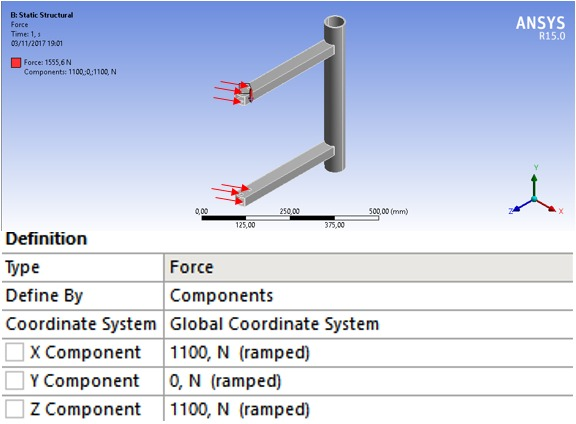
\includegraphics[scale=0.7]{figuras/forcas_1}
        \captionof{figure}{Aplicação das forças}
        \label{forcas_1}
    \end{center}   
    %Figura 4: Aplicação das forças
     
    
    \begin{center}
    	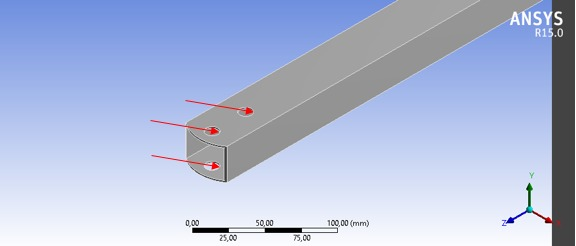
\includegraphics[scale=0.7]{figuras/forcas_2}
        \captionof{figure}{Aplicação das forças em escala aumentada}
        \label{forcas_2}
    \end{center}  
    %Figura 5: Aplicação das forças em escala aumentada
 
    Com as forças definidas foram feitas as simulações no cavalete pois ele é o componente estrutural e que sustenta a maior carga, sendo ela a junção do peso da bicicleta e do jogador e suas energias consequentes.
 
    Para a parte traseira foram divididas em 2 partes:
    \begin{itemize}
        \item Simulações na peça sem rolo do cavalete – Peça 1.
        \item Simulações na peça com rolo do cavalete – Peça 2.
    \end{itemize}
 
    \begin{center}
    	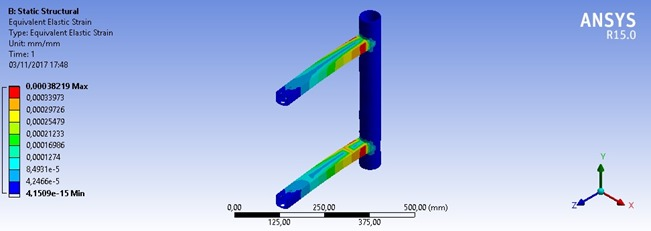
\includegraphics[scale=0.7]{figuras/sim_estatica_3}
        \captionof{figure}{Simulação estática peça 1 – Tensão elástica equivalente}
        \label{sim_estatica_3}
    \end{center}
    % Figura 6: Simulação estática peça 1 – Tensão elástica equivalente
    
    \begin{center}
    	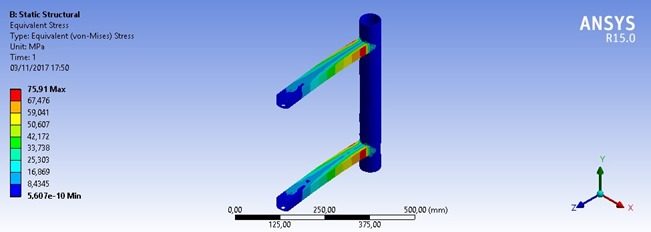
\includegraphics[scale=0.7]{figuras/stress_3}
        \captionof{figure}{Stress equivalente com Tensão de escoamento da peça 1}
        \label{stress_3}
    \end{center}
    %Figura 7: Stress equivalente peça 1 com Tensão de escoamento
    
    \begin{center}
    	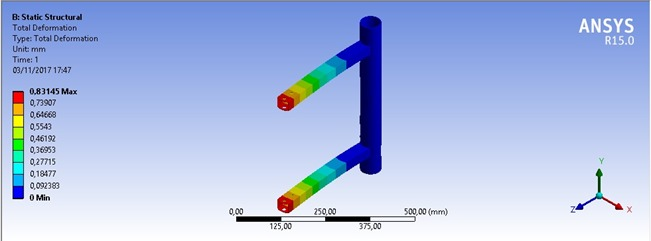
\includegraphics[scale=0.7]{figuras/deformacao_1}
        \captionof{figure}{Total deformação da peça 1}
        \label{deformacao_1}
    \end{center}
    %Figura 8: Total deformação da peça 1

    \begin{center}
    	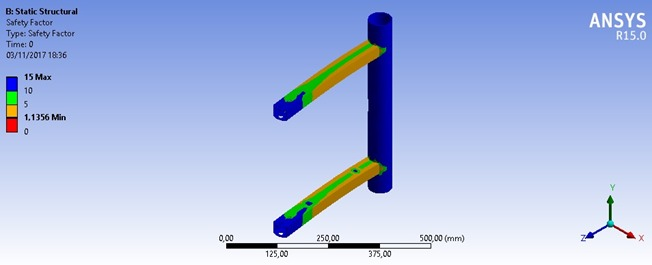
\includegraphics[scale=0.7]{figuras/fator_seguranca_3}
        \captionof{figure}{Fator de Segurança da peça 1}
        \label{fator_seguranca_3}
    \end{center}
    %Figura 9: Fator de segurança da peça 1
    
    \begin{center}
    	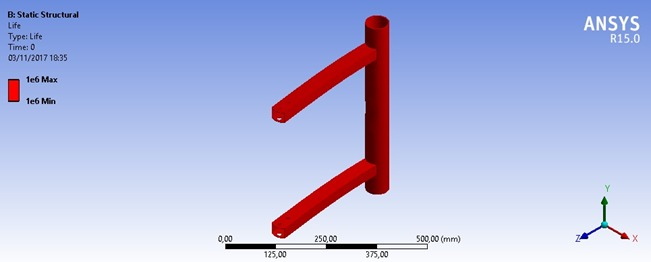
\includegraphics[scale=0.7]{figuras/vida_util_3}
        \captionof{figure}{Vida útil da peça 1}
        \label{vida_util_3}
    \end{center}
    %Figura 10: Vida útil da peça 1

    \begin{center}
    	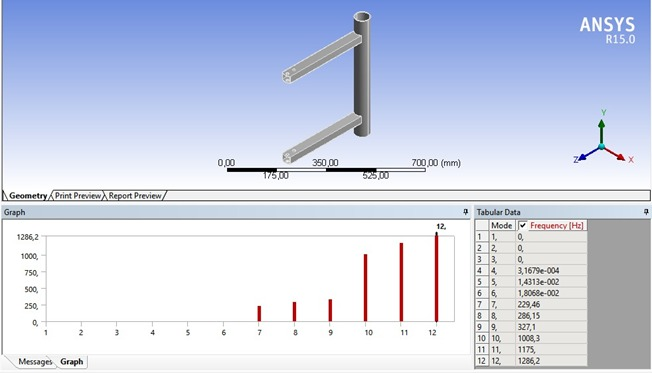
\includegraphics[scale=0.7]{figuras/vibracao_1}
        \captionof{figure}{Modos de vibração de ressonância da peça 1}
        \label{vibracao_1}
    \end{center}    
    %Figura 11: Modos de vibração de ressonância da peça 1
 
    Como pode ser observado, todos os testes validam a peça para fabricação:
    \begin{itemize}
        \item A figura \ref{sim_estatica_3} mostra a deformação elástica (em mm) que a peça 1 sofre com a carga aplicada, esta deformação é considerada nula;
        \item A figura \ref{stress_3} mostra a tensão de escoamento que o material da peça 1 alcança (75,91 MPa), sendo muito inferior a tensão de escoamento do aço 1045 (310 Mpa);
        \item A figura \ref{deformacao_1} mostra a deformação total da peça 1, considerada nula.
        \item A figura \ref{fator_seguranca_3} mostra o Fator de segurança da peça 1 pelas condições de contorno, sendo esse fator igual a 15;
        \item A figura \ref{vida_util_3} mostra a vida útil da peça 1 tendo como resultado uma peça com vida útil muito grande.
        \item A figura \ref{vibracao_1} mostra os módulos de vibração da peça 1, vemos que os 6 primeiros modos de vibração são considerados nulos, para que a faça com que a estrutura entre em ressonância é necessário chegar ao sétimo modo de vibração de 229,46 Hz, sendo que para a aplicação desta estrutura tal frequência jamais será alcançada.
    \end{itemize}
    
    A peças 1 suporta com segurança os esforços nela aplicado.
 
    Para a peça 2 foram feitas tais simulações:
 

    \begin{center}
    	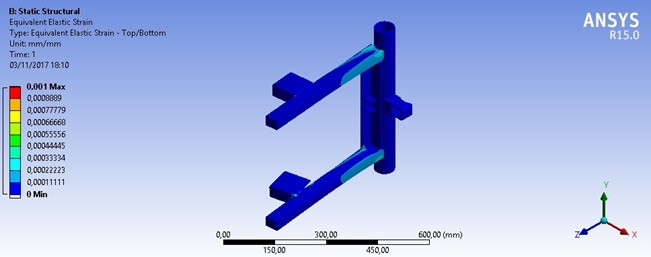
\includegraphics[scale=0.7]{figuras/sim_estatica_4}
        \captionof{figure}{Simulação estática peça 2 – Tensão elástica equivalente}
        \label{sim_estatica_4}
    \end{center}
    % Figura 6: Simulação estática peça 2 – Tensão elástica equivalente
    
    \begin{center}
    	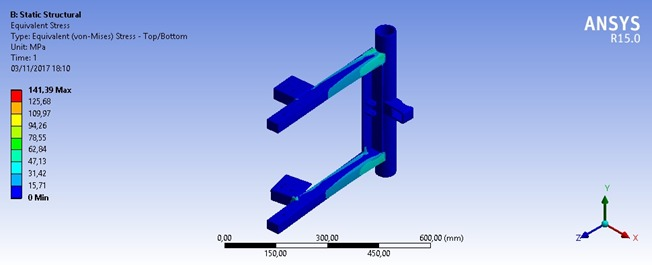
\includegraphics[scale=0.7]{figuras/stress_4}
        \captionof{figure}{Stress equivalente com Tensão de escoamento da peça 2}
        \label{stress_4}
    \end{center}
    %Figura 7: Stress equivalente peça 2 com Tensão de escoamento
  
    \begin{center}
    	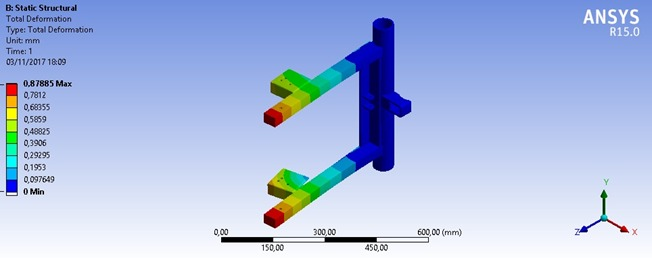
\includegraphics[scale=0.7]{figuras/deformacao_2}
        \captionof{figure}{Modal de corpo livre - deformação total da peça 2}
        \label{deformacao_2}
    \end{center}
    %Figura 8: Total deformação da peça 2    

    \begin{center}
    	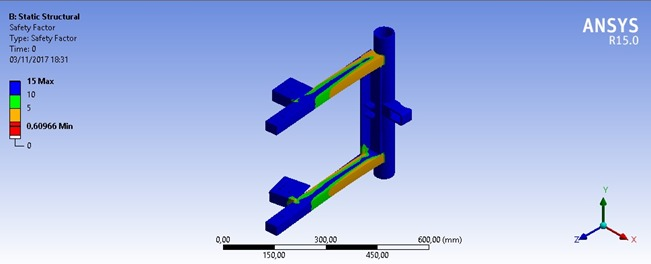
\includegraphics[scale=0.7]{figuras/fator_seguranca_4}
        \captionof{figure}{Fator de Segurança da peça 2}
        \label{fator_seguranca_4}
    \end{center}
    %Figura 9: Fator de segurança da peça 2
    
    \begin{center}
    	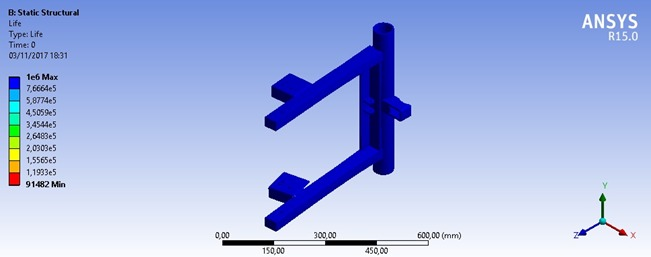
\includegraphics[scale=0.7]{figuras/vida_util_4}
        \captionof{figure}{Vida útil da peça 2}
        \label{vida_util_4}
    \end{center}
    %Figura 10: Vida útil da peça 2

    \begin{center}
    	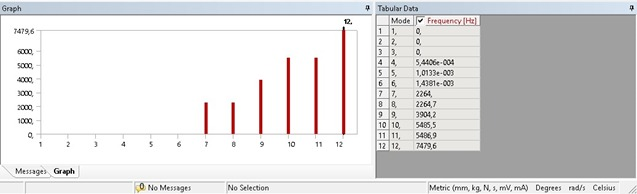
\includegraphics[scale=0.7]{figuras/vibracao_2}
        \captionof{figure}{Modos de vibração de ressonância da peça 2}
        \label{vibracao_2}
    \end{center}    
    %Figura 11: Modos de vibração de ressonância da peça 1

    Como pode ser observado, todos os testes também validam a peça para fabricação:
 
    \begin{itemize}
        \item A figura \ref{sim_estatica_4} mostra a deformação elástica (em mm) que a peça 2 sofre com a carga aplicada, esta deformação é considerada nula;
        \item A figura \ref{stress_4} mostra a tensão de escoamento que a peça 2 alcança (141,39 MPa), sendo também muito inferior a tensão de escoamento do aço 1045 (310 Mpa);
        \item A figura \ref{deformacao_2} mostra a deformação total da peça 2, considerada mínima.
        \item A figura \ref{fator_seguranca_4} mostra o Fator de segurança da peça 2 pelas condições de contorno, sendo esse fator também igual a 15;
        \item A figura \ref{vida_util_4} mostra a vida útil da peça 2 tendo como resultado uma peça com vida útil muito grande.
        \item Assim como a peça 1 a peça 2 possui os 6 primeiros modos e para chegar na frequência natural da peça seria necessário alcançar 2264 Hz, inalcançável considerando a sua aplicação
    \end{itemize}

A peça 2 também está válida para o uso.

\subsection{Suporte do Rolo}

Suporte do rolo (figura \ref{esq_suporte_rolo_1} e figura \ref{esq_suporte_rolo_2}), fica acoplado na estrutura traseira e suporta o rolo.
 
    \begin{center}
    	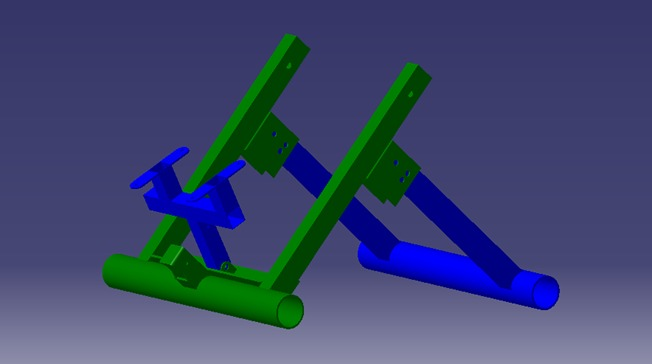
\includegraphics[scale=0.7]{figuras/esq_suporte_rolo_1}
        \captionof{figure}{Esquema estrutura parte traseira com suporte do rolo}
        \label{esq_suporte_rolo_1}
    \end{center} 

%Figura 1: Esquema estrutura parte traseira com suporte do rolo
 
    \begin{center}
    	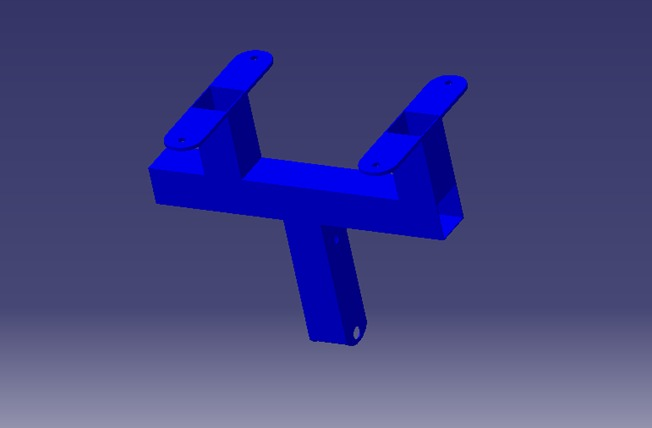
\includegraphics[scale=0.7]{figuras/esq_suporte_rolo_2}
        \captionof{figure}{Esquema estrutura completa de acoplamento parte traseira.}
        \label{esq_suporte_rolo_2}
    \end{center} 
%Figura 2: Esquema estrutura completa de acoplamento parte traseira.
 
Para calcular os esforços para as simulações, foram usados os cálculos apresentados na “figura \ref{analise_corpos_livres} - Análise Corpos Livres”.  Foi utilizado a força total aplicada na estrutura traseira nos dois suportes do rolo e dividida simultaneamente para a superfície de contado do rolamento em vermelho na Figura 3.

    \begin{center}
    	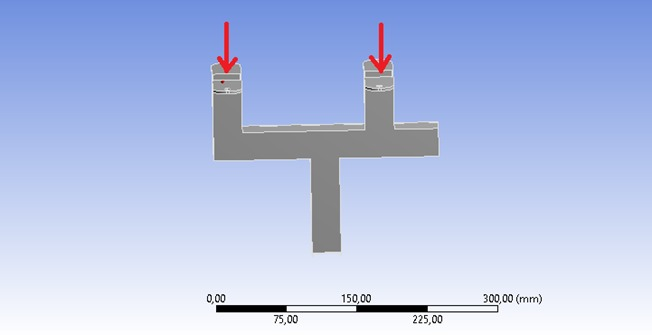
\includegraphics[scale=0.7]{figuras/forcas_3}
        \captionof{figure}{Aplicação das forças no suporte.}
        \label{forcas_3}
    \end{center} 
%Figura 3: Aplicação das forças no suporte.
  
Com as forças definidas foram feitas as simulações no suporte.
    \begin{center}
    	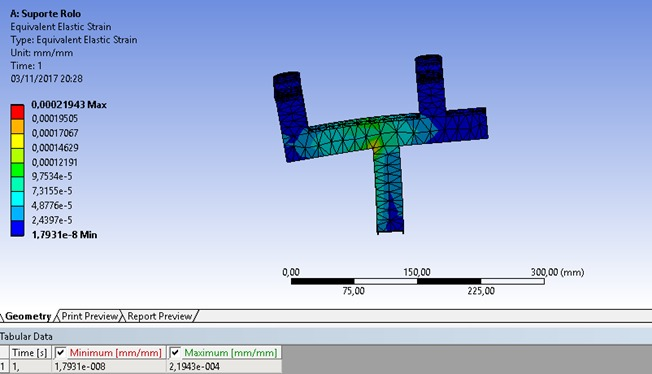
\includegraphics[scale=0.7]{figuras/sim_estatica_5}
        \captionof{figure}{Simulação estática do suporte – Tensão elástica equivalente}
        \label{sim_estatica_5}
    \end{center} 
%Figura 4: Simulação estática do suporte – Tensão elástica equivalente
     \begin{center}
    	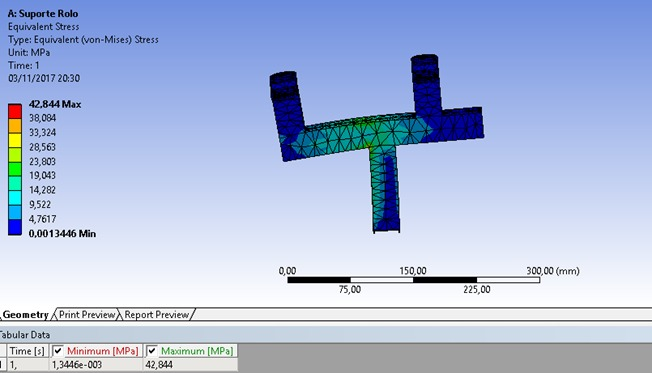
\includegraphics[scale=0.7]{figuras/stress_5}
        \captionof{figure}{Stress equivalente com Tensão de escoamento do suporte.}
        \label{stress_5}
    \end{center} 
%Figura 5: Stress equivalente com Tensão de escoamento do suporte.
    \begin{center}
    	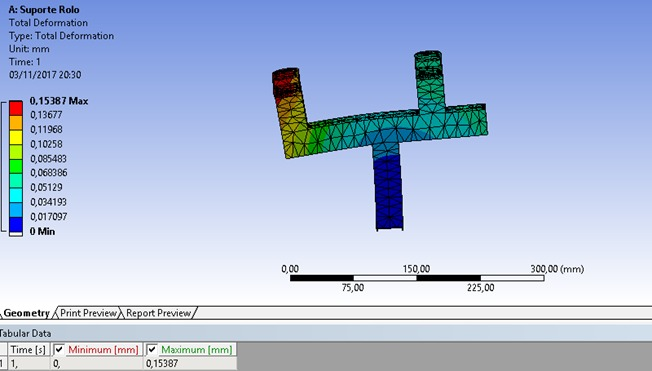
\includegraphics[scale=0.7]{figuras/deformacao_3}
        \captionof{figure}{Total deformação do suporte.}
        \label{deformacao_3}
    \end{center} 
%Figura 6: Total deformação do suporte.
     \begin{center}
    	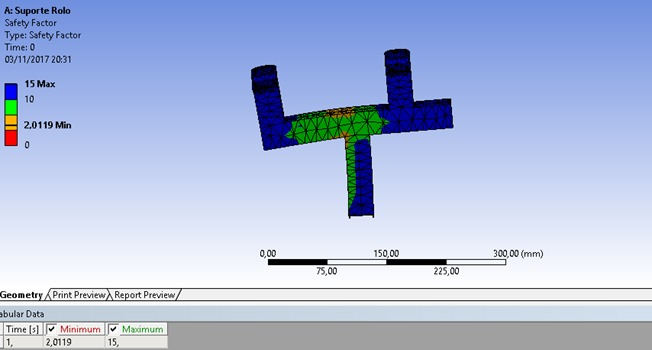
\includegraphics[scale=0.7]{figuras/fator_seguranca_5}
        \captionof{figure}{Fator de segurança do suporte.}
        \label{fator_seguranca_5}
    \end{center} 
%Figura 7: Fator de segurança do suporte.
    \begin{center}
    	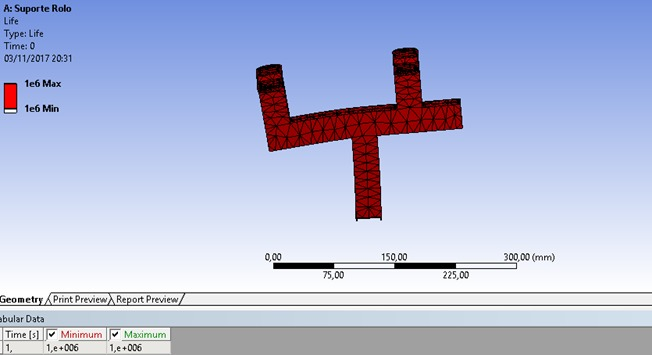
\includegraphics[scale=0.7]{figuras/vida_util_5}
        \captionof{figure}{Vida útil do suporte.}
        \label{vida_util_5}
    \end{center} 
%Figura 8: Vida útil do suporte.
    \begin{center}
    	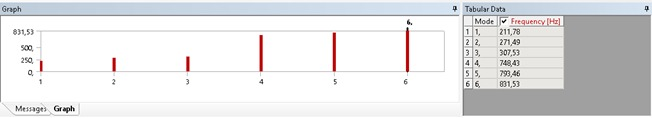
\includegraphics[scale=0.7]{figuras/vibracao_3}
        \captionof{figure}{Modos de vibração de ressonância do suporte.}
        \label{vibracao_3}
    \end{center} 
%Figura 9: Modos de vibração de ressonância do suporte.
 
Como pode ser observado, todos os testes validam a peça para o uso:
\begin{itemize}
    \item A figura \ref{sim_estatica_5} mostra a deformação elástica (em mm) que o suporte sofre com a carga aplicada, esta deformação é considerada nula;
    \item A figura \ref{stress_5} mostra a tensão de escoamento que o material do suporte alcança (42,844 MPa), sendo muito inferior a tensão de escoamento do aço 1045 (310 Mpa);
    \item A figura \ref{deformacao_3} mostra a deformação total do suporte, considerada mínima.
    \item A figura \ref{fator_seguranca_5} mostra o Fator de segurança do suporte pelas condições de contorno, sendo esse fator igual a 15;
    \item A figura \ref{vida_util_5} mostra a vida útil do suporte tendo como resultado uma peça com vida útil muito grande.
    \item A figura \ref{vibracao_3} mostra os módulos de vibração do suporte, vemos que o primeiro modo de vibração de 211,78 Hz é inalcançável devido as aplicações da estrutura.
\end{itemize}

O Suporte de rolo é valido com segurança para os esforços nela aplicado.

\subsection{Freio controlado} 
    Esse componente tem como objetivo dificultar a pedalada em simulação de subida e liberar na descida e plano para aumentar a imersão da realidade aumentada.

    A primeira versão dessa solução foi fazer o controle por meio do alternador que seria também utilizado para gerar energia. Ela seria conectada na coroa ao lado do rolo por uma correia.

    Esta solução não deu certo pelas complicações causadas pelo alternador. Seria difícil gerar energia e ao mesmo tempo dificultar e liberar a pedalada. Os testes feitos mostraram complicações em nível mais fundamental com esse equipamento, o que fez descartar essa solução (mais informações verificar a sessão que trate desse tema).

    A segunda solução que tivemos foi fazer um sistema com disco de freio de moto, porém com teste, verificou-se que era sensível demais e que causaria uma carga muito alta rapidamente, portanto excluiu-se tal solução.

    \begin{center}
    	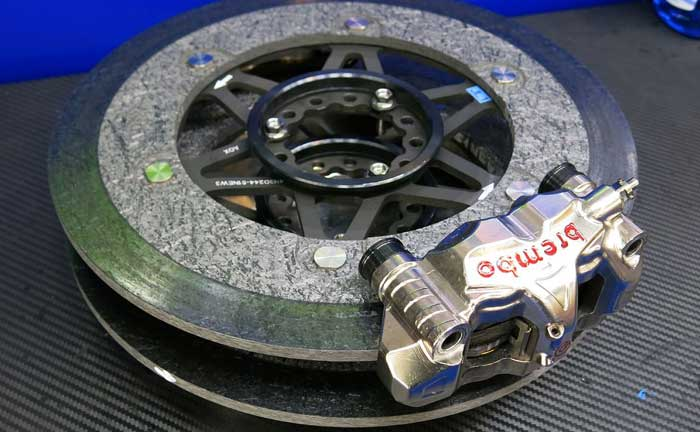
\includegraphics[scale=0.5]{figuras/freio_moto}
        \captionof{figure}{Freio a disco de moto.}
        \label{freio_moto}
    \end{center} 
    %Figura X: Freio a disco de moto

    A terceira solução foi utilizar um espécie de pêndulo com uma mola que seria puxado para encostar na parte não utilizada da coroa para causar certo atrito e aumentar a carga assim. Essa solução acabou sendo substituída devido a incerteza e insegurança quanto a funcionalidade e projetação dessa alternativa.

    \begin{center}
    	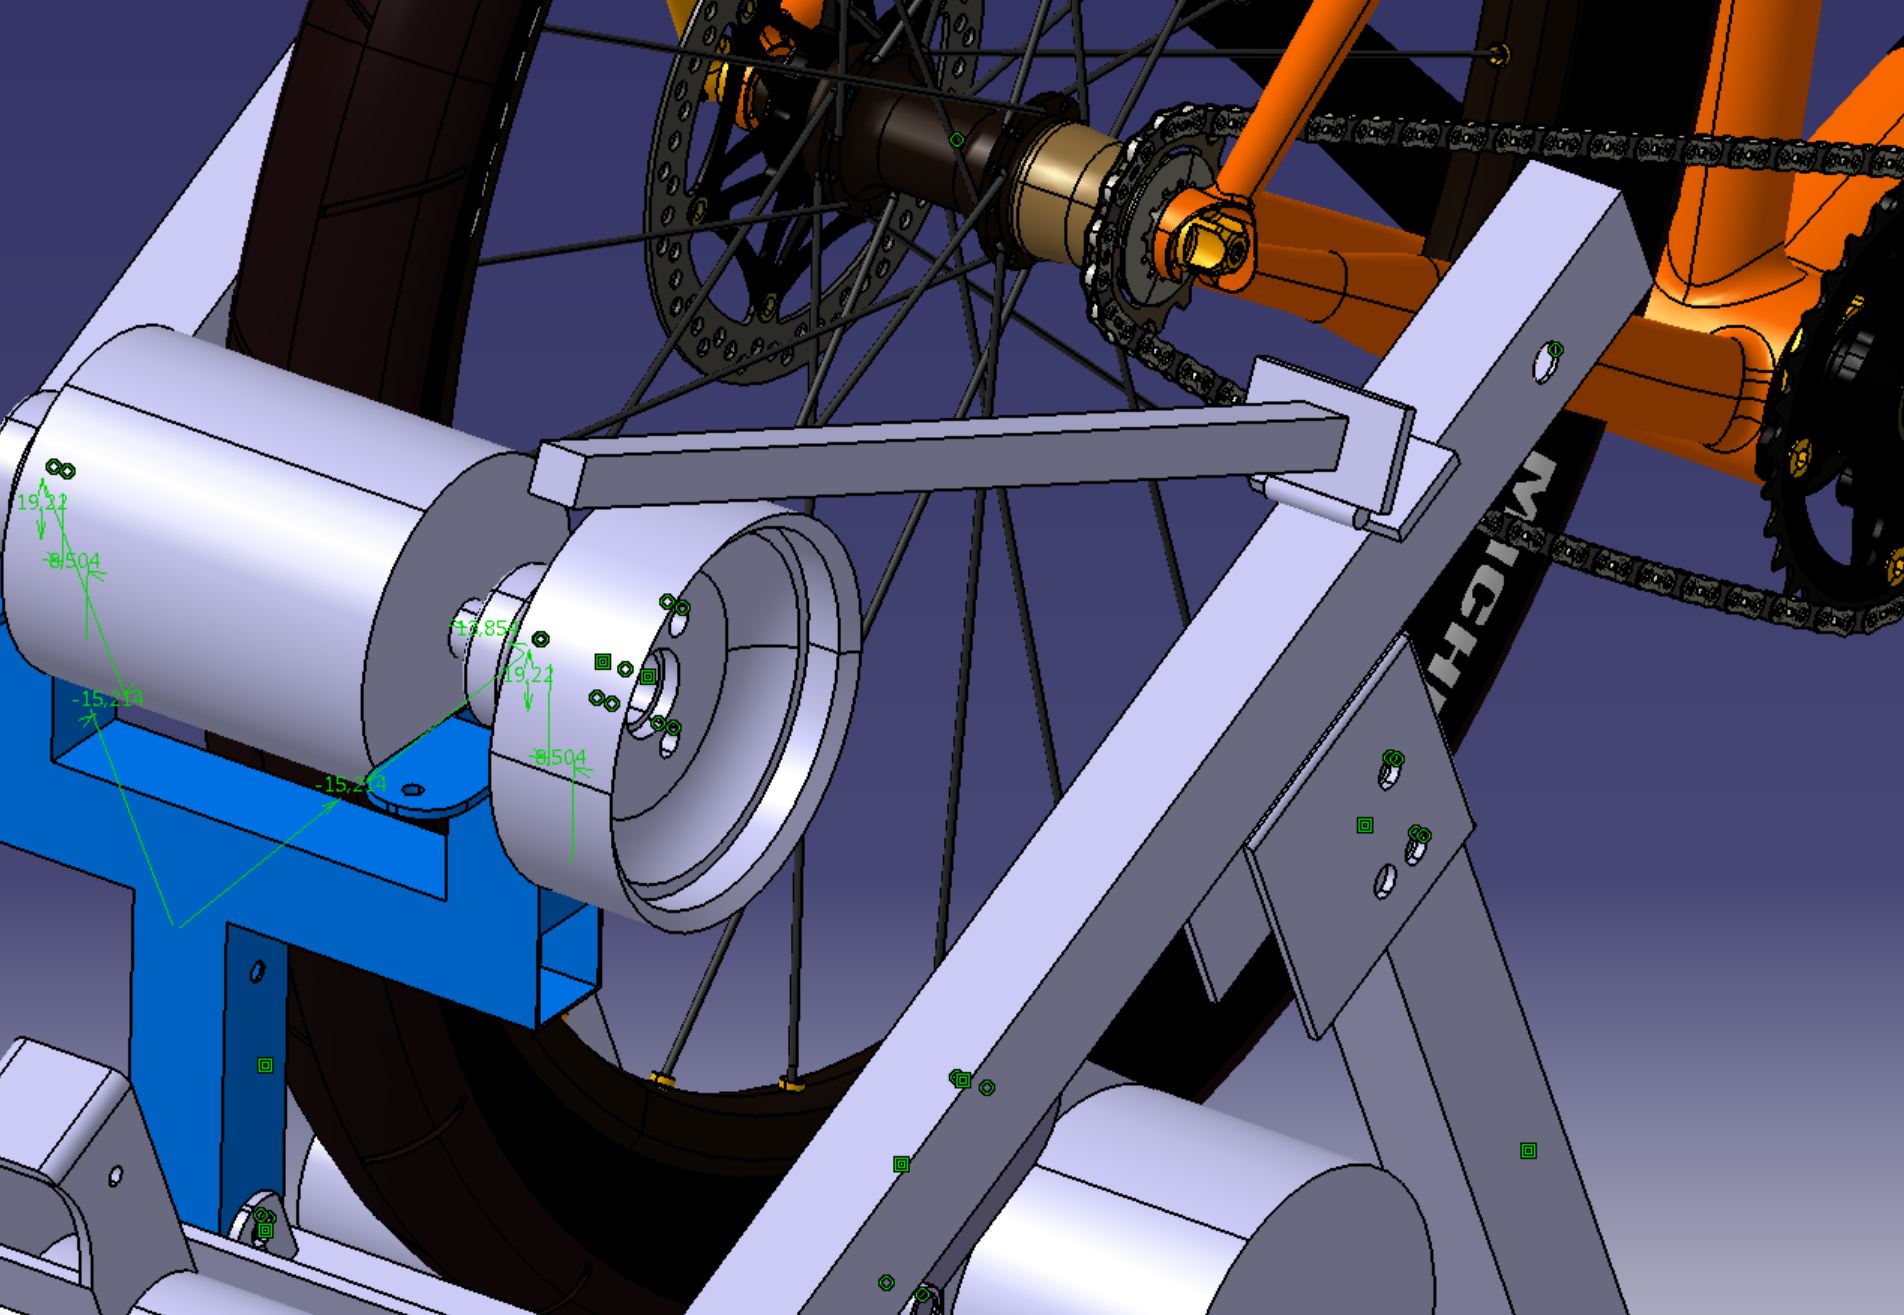
\includegraphics[scale=0.5]{figuras/freio_pendulo}
        \captionof{figure}{Freio com pêndulo}
        \label{freio_pendulo}
    \end{center} 
    %Figura X: Freio com pêndulo

    A quarta solução foi utilizar um freio a disco de bicicleta preso no eixo do rolo. Essa solução se demonstrou ser a mais profissional, por já ser bem usada no mercado, de fácil acesso e projetação mais direta. Foram feitas várias alternativas para essa solução, mas a final está representada abaixo.

    \begin{center}
    	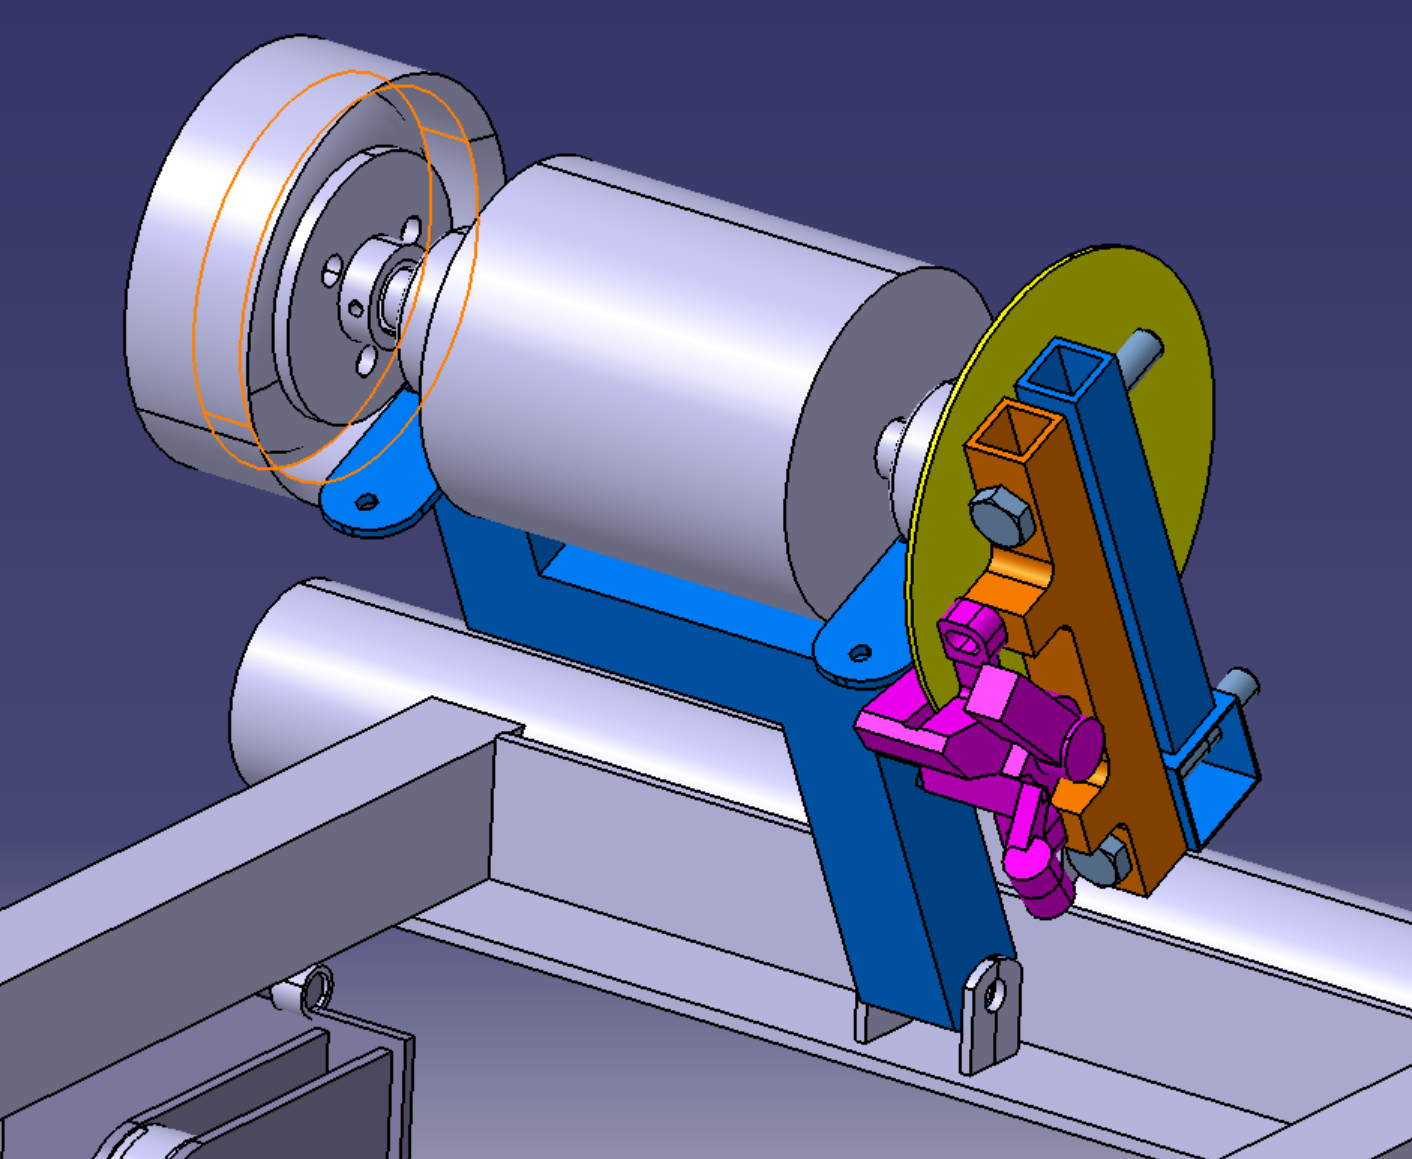
\includegraphics[scale=0.5]{figuras/carga_peso}
        \captionof{figure}{Sistema de carga de peso na simulação. Em amarelo, o disco de freio, em rosa, a pinça para frear, em laranja a estrutura de fixação da pinça e em azul o suporte do rolo.}
        \label{carga_peso}
    \end{center} 
    %Figura X: Sistema de carga de peso na simulação. Em amarelo, o disco de freio, em rosa, a pinça para frear, em laranja a estrutura de fixação da pinça e em azul o suporte do rolo.

    Esta alternativa foi encontrada depois de utilização de vários iterações de simulações estruturais e CADs. Algumas coisas percebidas foram o tamanho adequado do tubo azul a ser soldado e a adição de mais um parafuso em cima da estrutura da pinça para garantir maior contato.  As simulações ainda alertaram para as regiões de maior estresse e maior deslocamento.

    \begin{center}
    	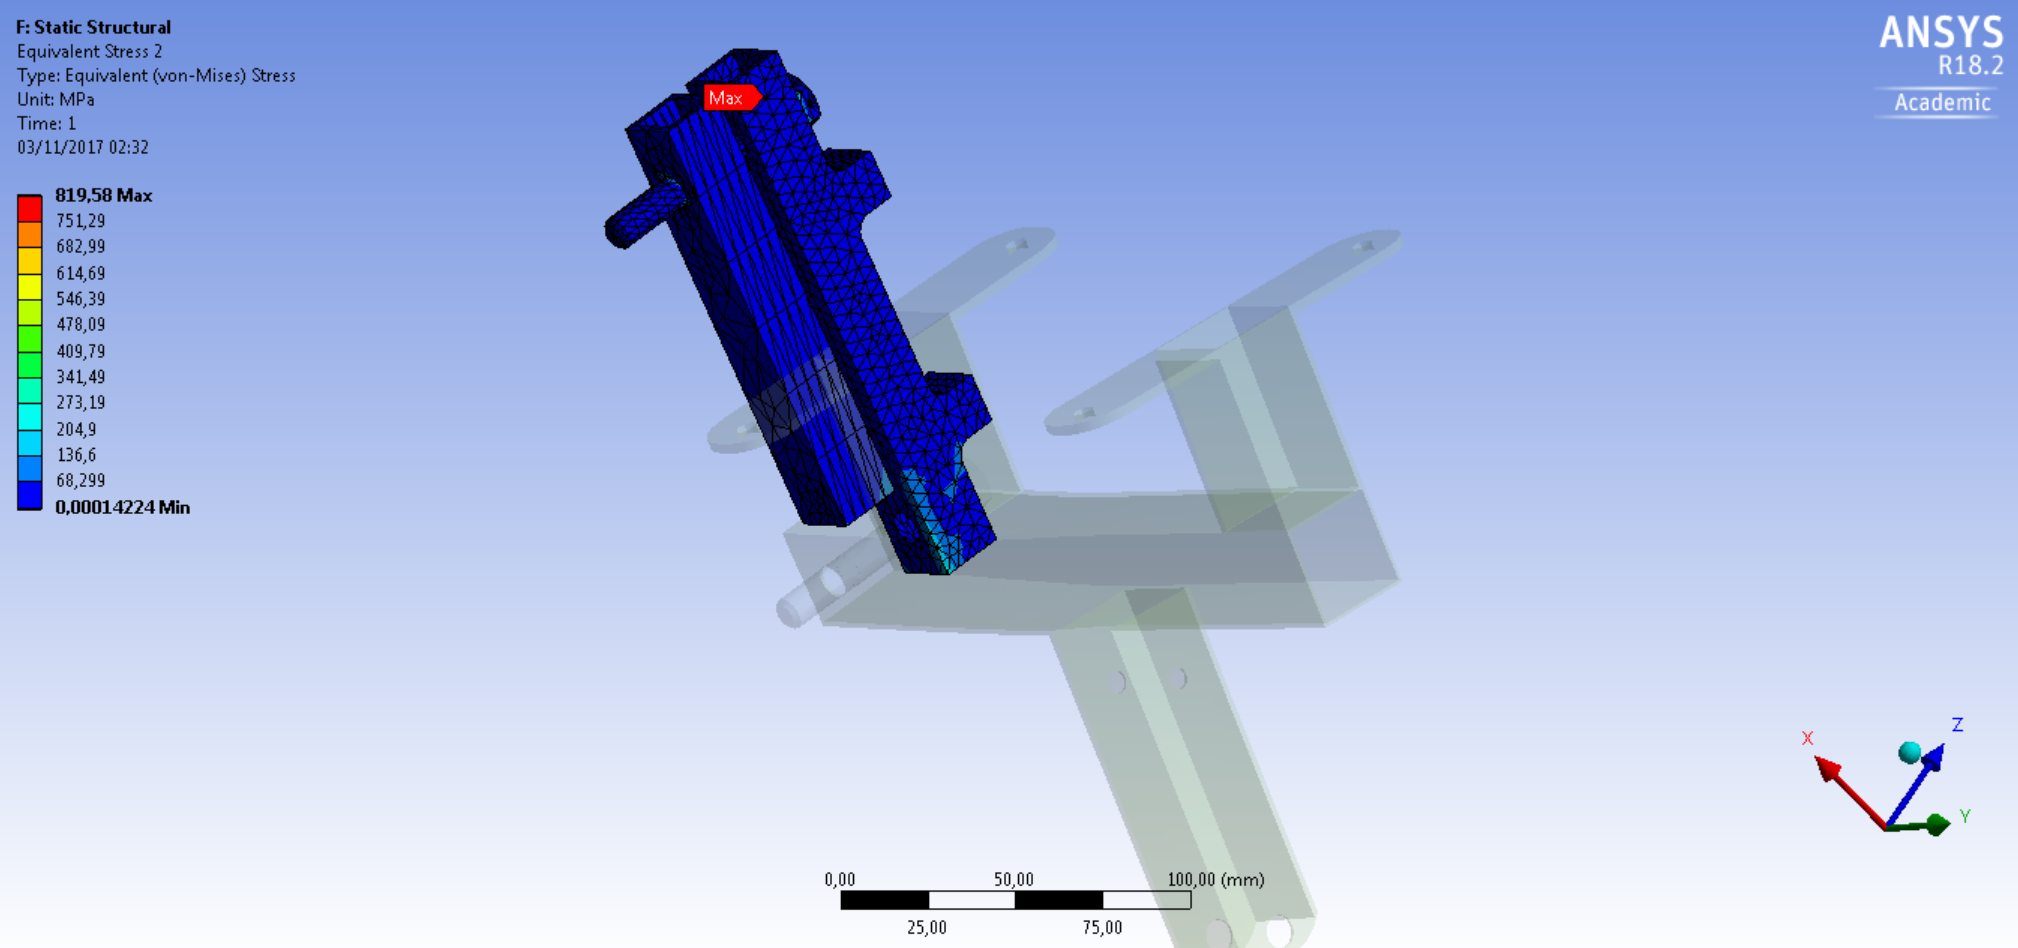
\includegraphics[scale=0.5]{figuras/sim_est_freio}
        \captionof{figure}{Simulação estrutural do sistema do freio.}
        \label{sim_est_freio}
    \end{center} 
    %Figura X: Simulação estrutural do sistema do freio.

    Na figura acima vê-se a tensão máxima como sendo de 800 MPA no parafuso, mas isso se deve uma descontinuidade no parafuso. As maiores tensões se encontram na parte inferior voltada para o rolo e nas regiões dos parafusos. Para resolver a primeira região será acrescentado cantoneiras e para a segunda, acrescentar-se-á buchas para aumentar a superfície de contato com o parafuso.

\subsection{Alternador}
 
    Como apresentado no relatório do sistema de alimentação, o alternador não funcionou como esperado e projetado, consumindo energia ao invés de gerar. Assim, o projeto da figura \ref{alternador} foi pausado e  será reestruturado para o novo alternador substituto

    \begin{center}
    	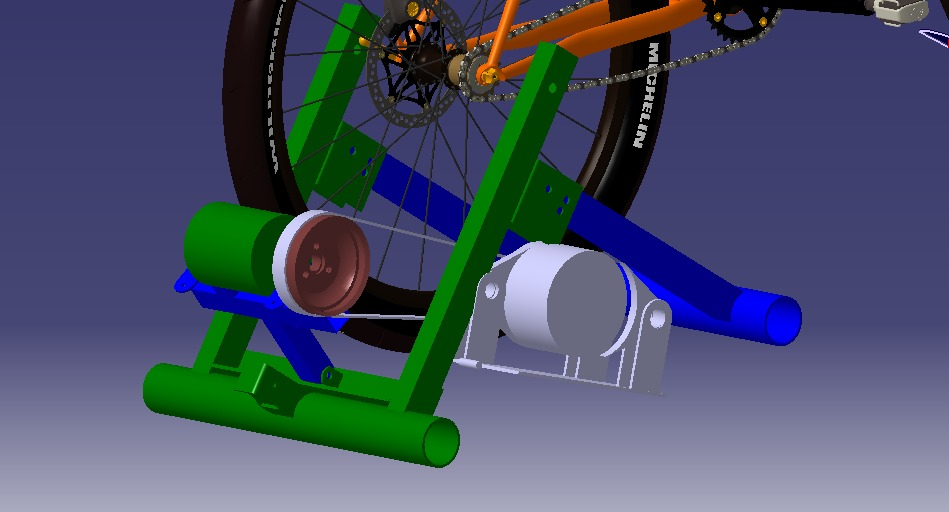
\includegraphics[scale=0.5]{figuras/alternador}
        \captionof{figure}{CAD do alternador com a correia acoplada na coroa}
        \label{alternador}
    \end{center} 